\documentclass{article}

\title{Algebraic Topology Homework 4}
\author{Adam Buskirk}

\usepackage{amssymb,amsmath,amsthm}
\usepackage{tikz}
\usetikzlibrary{trees}
\usetikzlibrary{matrix}
\usepackage[margin=1in]{geometry}

\newtheorem{theorem}[subsection]{Theorem}
\newtheorem{conjecture}[subsection]{Conjecture}
\newtheorem{lemma}[subsection]{Lemma}
\theoremstyle{definition}
\newtheorem{definition}[subsection]{Definition}

\newcommand{\R}{\mathbb{R}}
\newcommand{\N}{\mathbb{N}}
\newcommand{\Q}{\mathbb{Q}}
\newcommand{\Z}{\mathbb{Z}}
\newcommand{\Co}{\mathbb{C}}
\newcommand{\p}[1]{\left(#1\right)}
\newcommand{\sq}[1]{\left[#1\right]}
\newcommand{\set}[1]{\left\{#1\right\}}
\newcommand{\norm}[1]{\left|\left|#1\right|\right|}
% \newcommand{\p}[1]{\left(#1\right)}

\begin{document}
\maketitle

\section{Problem 2}
\begin{theorem}
Let $X=\R^{n+1} \setminus \{0\}$; define an equivalence relation on 
$\sim$ on $X$ where $x \sim y$ iff $x=\lambda y$ for some $\lambda \in \R^+$.
Then $S^n \cong X/\sim$. Furthermore we can define another equivalence
relation $\bumpeq$ on $S^n$ by identifying antipodal points and show that
$S^n/\bumpeq \cong \R P^n$.
\end{theorem}
\begin{proof}
Let $q : x \mapsto [x]_\sim$ be the quotient map which takes each element of
$\R^{n+1} \setminus\{0\}$ to its equivalence class under $\sim$, and let 
$f : X \to S^n$, $f : x \mapsto \frac{1}{|x|} x$.
{\begin{center}
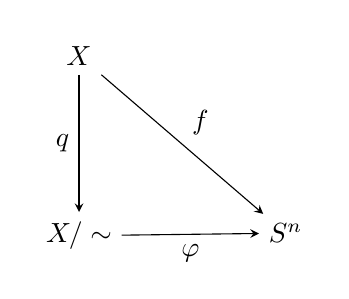
\begin{tikzpicture}[every node/.style={midway},->,>=stealth]
        \matrix (m) [matrix of math nodes, column sep={5em}, row sep={5em}]
        {
                X & \\
                X / \sim & S^n
        \\};
        \draw[->] (m-1-1) -- (m-2-2) node[above right] {$f$} ;
        \draw[->] (m-1-1) -- (m-2-1) node[left] {$q$};
        \draw[->] (m-2-1) -- (m-2-2) node[below] {$\varphi$};
\end{tikzpicture}
\end{center}}
The map $f$ is constant on the fibers of $q$, since if $f(x_1) = f(x_2)$ then
$x_1/|x_1|=x_2/|x_2|$, which implies $x_1 = \frac{|x_1|}{|x_2|} x_2$, meaning
$x_1 \sim x_2$ and thus $q(x_1) = q(x_2)$. On the other hand, if 
$q(x_1)=q(x_2)$ then $x_1=\lambda x_2$, so $|x_1|=\lambda |x_2|$ which
implies $\lambda = \frac{|x_1|}{|x_2|}$ and thus 
$x_1 = \frac{|x_1|}{|x_2|} x_2$ and so 
$f(x_1) = x_1/|x_1| = x_2 / |x_2| = f(x_2)$.
Thus by Theorem 3.75
there must exist a homeomorphism $\varphi : X/\sim \to S^n$, and thus
$X/\sim$ and $S^n$ are homeomorphic.

Similarly, if we let $g$ map each point in $X$ to its equivalence class
in $\R P^n$, and let $p$ map each point of $S^n$ to the equivalence class
of antipodal points defined by $\bumpeq$, we have 
{\begin{center}
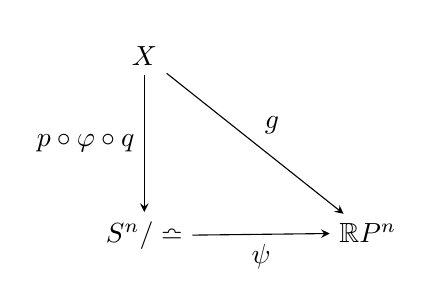
\begin{tikzpicture}[every node/.style={midway},->,>=stealth]
        \matrix (m) [matrix of math nodes, column sep={5em}, row sep={5em}]
        {
                X & \\
                S^n/\bumpeq & \R P^n
        \\};
        \draw[->] (m-1-1) -- (m-2-2) node[above right] {$g$} ;
        \draw[->] (m-1-1) -- (m-2-1) node[left] {$p\circ \varphi \circ q$};
        \draw[->] (m-2-1) -- (m-2-2) node[below] {$\psi$};
\end{tikzpicture}
\end{center}}
If $g(x_1) = g(x_2)$ then $x_1 = \lambda x_2$ so 
$|x_1| = |\lambda| \cdot |x_2|$ so $|\lambda| = \frac{|x_1|}{|x_2|}$. 
Hence $x_1 = s\frac{|x_1|}{|x_2|} x_2$ for some $s \in \{-1,1\}$, whichever
is appropriate. If $s=1$, then $\varphi \circ q = f$ maps $x_1$ and $x_2$
to the same element, and thus 
$p \circ \varphi \circ q (x_1) = p \circ \varphi \circ q (x_2)$. $s=-1$, then
they map to opposite points on the sphere, which are in the same equivalence
class, and thus the same equality holds. 

If $p \circ \varphi \circ q (x_1) = p \circ \varphi \circ q (x_2)$, then 
$\varphi \circ q (x_1) = \pm \varphi \circ q (x_2)$ which is the same
as $f (x_1) = \pm f(x_2)$ and thus $x_1/|x_1| = \pm x_2 / |x_2|$, so 
$x_1 = \pm \frac{|x_1|}{|x_2|} x_2$ so $x_1 \bumpeq x_2$ and thus
$g(x_1) = g(x_2)$.

Since both maps agree on fibers, by 3.75 there exists a homeomorphism 
$\psi$ between $S^n / \bumpeq$ and $\R P^n$.
\end{proof}

\section{Problem 3}
\begin{theorem}
Let $X=\R \times \{0,1\}$, and let $\sim$ such that $(x,1) \sim (y,0)$ iff 
$x=y \neq 0$. Therefore, the classes $[(0,0)]$ and $[(0,1)]$ are distinct.
Then $X / \sim$ is second countable, locally Euclidean, but not Hausdorff.
\end{theorem}
\begin{proof}
(Locally Euclidean) 
% Let $f$ be the quotient map associated with $\sim$. Observe first that 
% $\pi_1$ agrees with $f$ on the fibers of $f$; if $f(x_1,x_2) = f(y_1,y_2)$,
% then we know $x_1=y_1$ and if those are zero, $x_2=y_2$. The first equation
% gives $\pi_1(x_1,x_2) = x_1 = y_1 = \pi_1(y_1,y_2)$. Thus we may pass 
% $\pi_1$ through the quotient to obtain a continuous map $\phi$.
% {\begin{center}
% \begin{tikzpicture}[every node/.style={midway},->,>=stealth]
%         \matrix (m) [matrix of math nodes, column sep={5em}, row sep={5em}]
%         {
%                 X & \\
%                 X /\sim & \R
%         \\};
%         \draw[->] (m-1-1) -- (m-2-2) node[above right] {$\pi_1$} ;
%         \draw[->] (m-1-1) -- (m-2-1) node[left] {$f$};
%         \draw[->] (m-2-1) -- (m-2-2) node[below] {$\phi$};
% \end{tikzpicture}
% \end{center}}
If $x \in X / \sim$, then $x_1 \in (a,b) \subseteq \R$. If
not both $x_1=0$ and $x_2=1$, 
then we assume that $0 \not\in(a,b)$; if so, then
$x\in(0,b)$ or $x\in(a,0)$ and proceed with that open neighborhood. 
Then $(a,b) \cong \{ [(x,0)] : a < x < b \}$ by the inclusion map, 
since $A \subseteq (a,b)$ is open implies $A \times \{0\}$ and
$A \times \{1\}$ are open in $X$, hence 
$\{[(x,0)] : x \in A \}$ is open since its preimage under $f$ is 
$A \times \{0,1\}$, the union of two open sets. Thus the image
of an arbitrary open set under 
$i : (a,b) \to \{[(x,0)] : a < x < b\}$ is open; so this inclusion
map is open. Furthermore, if $B \subseteq \{[(x,0)] : a < x < b\}$ 
is open, then $B$'s preimage is the set of $x \in (a,b)$
indexing $B$, which will be open. Hence $i$ is continuous.
It is also bijective (injective since 
each $p \in (a,b)$ is mapped
to the unique element $[(p,0)]$ in the open subset of $X / \sim$, and
since each element of the open image is indexed by exactly one element
of $(a,b)$, the mapping is surjective also). Consequently, $i$
is a bijective continuous open map, and thus $i$ is a homeomorphism
between $(a,b)$ a subset of $\R$ and an open neighborhood of $x$.

An open neighborhood around $[(0,1)]$ (the only point not yet
accounted for) homeomorphic to an open 
neighborhood of $\R$ is obtained by applying the homeomorphism
\[
P(x,y) = (x,1-y)
\]
which takes $(0,1)$ to $(0,0)$, which has an open neighborhood
homeomorphic to an open neighborhood of $\R$, which can be pulled
back through $P^{-1}$ to obtain an open neighborhood of $(0,1)$
homeomorphic to an open neighborhood of $\R$.

(Second countable) 
$M$ is a locally Euclidean quotient space of a 
second countable space $\R \times \{0,1\}$ ($X = \R \sqcup \R$ and 
proposition 3.42.e), and thus is also 
second countable by Proposition 3.56.

(Not Hausdorff) 
However, $X / \sim$ is not Hausdorff, since we cannot find disjoint 
open neighborhoods around $[(0,0)]$ and $[(0,1)]$. The preimage of a neighborhood
of $[(0,0)]$ must contain some open interval $(a,b) \times \{0\}$,
$a < 0 < b$,
and also the preimage of a neighborhood of $[(0,1)]$ must contain
some $(c,d) \times \{1\}$, $c < 0 < d$. However, consider the points 
$(\min(b,d)/2,0)$ and $(\min(b,d)/2,1)$; since neither $b$ nor $d$ can
be $0$, these must map to the same point under the quotient map. 
Consequently, the neighborhoods around $[(0,0)]$ and $[(0,1)]$ are
not disjoint; but they were chosen arbitrarily, and thus disjoint
open neighborhoods for these points in $X / \sim$ cannot be found.
Consequently, $X / \sim$ is not Hausdorff.
\end{proof}

\section{Problem 4}
\subsection{Example 2}
(Locally connected)
Observe that we cannot find any two disjoint nonempty sets $A,B$ in $\R_c$;
if we picked any two, then their intersection would exclude $A^C \cup B^C$,
which is also countable, and hence $A \cap B$ would be uncountable and thus
nonempty.
Hence every open subset of $\R_c$ is connected, and obviously the entire topology
of $\R_c$
is a basis for the space. Furthermore, we can find a 
basis of connected open sets for $[0,1]$. Hence the box basis obtained on 
$\R_c \times [0,1]$ by these is a basis of connected open subsets (Prop 3.31.d), 
and thus each of these sets in $\R_c \times [0,1] / \sim$ is still connected 
(Thm 4.7). The image of this basis is then a basis for $\R_c\times[0,1]/\sim$
and thus this is a locally connected space.

(Path connected)

(Connected) 
Implied by path connected.

(Not locally path-connected)
Notice that the only path-connected subsets of $\R_c$ are $\R_c$ itself and,
trivially, the empty set. Otherwise, some $p$ must be omitted, which prevents
a path in the set connecting $a$ and $b$ for any $a<p<b$ (some must exist, or
the set would not be cocountable). Thus if we suggested $\mathcal{B}$ was a 
basis for the set, then it must provide a basis element for 
$\p{\R_c-\set{0}} \times [0,0.5)$ which is homeomorphic to its image in the
quotient space (since it is bijective on this domain. Then if $U$ is a basis
element associated with the set above, and $a,b \in U$ are selected such that
$a_1 < 0 < b_1$, then if $f : I \to U$ is designated such that $f(0)=a$,
$f(1)=b$, then at some point $\pi_1 \circ f (x) = 0$, which would imply $U$
contained a point $f(x)$ outside of $\p{\R_c-\set{0}} \times [0,0.5)$, 
a contradiction. Hence no basis of path-connected sets may be found for 
the space, and thus it is not locally path-connected. 

\section{Problem 5}
\begin{theorem}
Manifolds have countably many connected components.
\end{theorem}
\begin{proof}
Suppose a manifold had uncountably many connected components. Since each
of these is an open set, for any basis for the manifold's topology, 
each of these connected components must contain a distinct basis
element. Thus an injection may be made from the uncountable collection
of components into any basis for the manifold, and thus any basis
for the manifold must be uncountable, contradicting the requirement
that a manifold be second-countable.
\end{proof}
\section{Problem 6}
\begin{theorem}
Let $G$ be a topological group and let $e$ denote the identity element. 
Let $H$ denote the connected component containing $e$. Then $H$ is a 
subgroup.
\end{theorem}
\begin{proof}
Consider arbitrary $g, h \in H$, and consider $\Phi_h : H \to G$ defined
by $\Phi_h ( k ) = kh^{-1}$. Then $\Phi_h$ is constructed from three 
different operations. First, $h \to h^{-1}$ is continuous by the definition
of a topological group. Also, the restriction of the product to $H \times H$
is continuous. So the composition $\phi : (j,k) \in H^2 \mapsto j \cdot k^{-1}G$ 
is continuous. So then $\Phi_h (k) = \phi(k,h)$ is continuous. Thus, since
continuous maps preserve connectivity by Theorem 4.7 in the text, we know that
$\Phi_h(H)$ is a connected set. Furthermore, 
$\Phi_h(h) = h h^{-1} = e \in \Phi_h(H)$,
so $\Phi_h(H) \subseteq H$; if not, $H$ would not be maximal, since 
$\phi_h(H) \cup H$ would then be a larger connected set not disjoint from $H$, 
and thus $H$ would not be considered a connected component of $G$. Since 
$g \in H$, the domain of $\Phi_h$, then 
$gh^{-1} = \Phi_h (g) \in \Phi_h (H) \subset H$, so $gh^{-1} \in H$. Thus,
$H$ is a subgroup of $G$.
\end{proof}

\end{document}
